
%       dvips -ta4 exercise03 -o
%       ps2pdf -sPAPERSIZE=a4 seddel03.ps

\documentclass[a4paper]{article}
\usepackage{times,fullpage}
\usepackage[latin1]{inputenc}
\usepackage[T1]{fontenc}
\usepackage{bprd}
\usepackage[dvips]{graphicx}
\usepackage{xcolor}
\usepackage{float}

\setcounter{exercise-sheet}{19}

\begin{document}

\begin{center}
{\Large\bf Exercises week \arabic{exercise-sheet}}\\[1ex]
%Monday 7 September 2009}\\[1ex]
%{\small 2009-09-09}\\[2ex]
\end{center}

\subsection*{Goal of the exercises}

The main goal of this week's exercises is to familiarize yourself with
regular expressions, automata, grammars, the \texttt{alex} lexer
generator and the \texttt{happy} parser generator.

%\noindent 
%Do exercises~\ref{exer-automata-mogensen}, \ref{exer-re},
%\ref{exer-expr-derivation}, \ref{exer-expr-derivation-tree},
%\ref{exer-expr-parse-try}, \ref{exer-expr-parse+scomp} and
%\ref{exer-expr-conditional}.  Hand in solutions to
%exercises~\ref{exer-re}, \ref{exer-expr-parse-try},
%\ref{exer-expr-parse+scomp} and~\ref{exer-expr-conditional}.
%Exercise~\ref{exer-expr-parse-steps} is very instructive too, but
%requires some patience.


%\begin{exercise}\label{exer-automata-mogensen}
%
%Do exercises 2.2 and 2.3 in Mogensen 2009.\\
%
%\noindent
%\textbf{\emph{Answer}} \\
%{\color{red}{I haven't translated this question/answer - not sure about its relevance?}}
%\end{exercise}


\begin{exercise}\label{exer-re}
  
  Write a regular expression that recognizes all sequences consisting
  of $a$ and $b$ where two $a$'s are always separated by at least one
  $b$.  For instance, these four strings are legal: $b$,\ \ $a$,\ \ 
  $ba$,\ \ $ababbbaba$; but these two strings are illegal: $aa$,\ \ 
  $babaa$.  \\

\noindent
\textbf{\emph{Answer}} 
{\codesetup\begin{verbatim}
   b+ | b*a(b+a)*b*
\end{verbatim}} 

  % Hint: either has no $a$'s at all, or it has an a, and if more a's
  % then one or more intervening b's; and may in any case have b's at the
  % ends: b* | b*a(b+a)*b*
 \noindent 
  Construct the corresponding NFA\@.  Try to find a DFA corresponding
  to the NFA. \\

\noindent
\textbf{\emph{Answer}} 
\begin{figure}[H]
  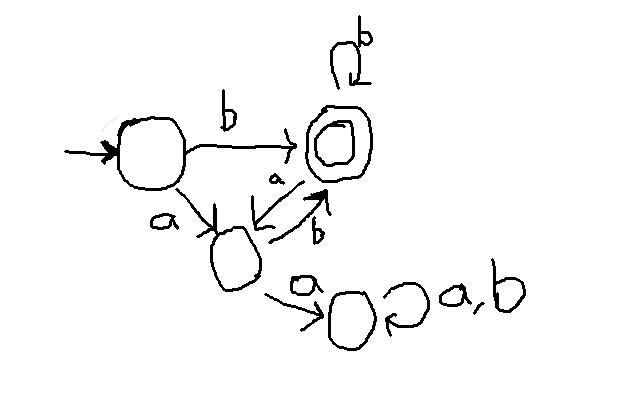
\includegraphics[width=10cm]{nfa.png}
\end{figure}
\end{exercise}


\begin{exercise}\label{exer-expr-derivation}
  Write out the rightmost derivation of this string from the
  expression grammar corresponding to \texttt{ExprLang/ExprPar.y}\@.  
  
{\codesetup\begin{verbatim}
   let z = 17 in z + 2 * 3 end 
\end{verbatim}} 

\noindent
  (Take note of the grammar rules (1 to 8) used:)
  
{\codesetup\begin{verbatim}
Expr    : var                          { Var  $1           } -- Rule 1
        | num                          { CstI $1           } -- Rule 2
        | '-' num                      { CstI (- $2)       } -- Rule 3
        | '(' Expr ')'                 { $2                } -- Rule 4
        | let var '=' Expr in Expr end { Let $2 $4 $6      } -- Rule 5
        | Expr '*' Expr                { Prim "*" $1 $3    } -- Rule 6
        | Expr '+' Expr                { Prim "+" $1 $3    } -- Rule 7
        | Expr '-' Expr                { Prim "-" $1 $3    } -- Rule 8
        
\end{verbatim}}  


\noindent
\textbf{\emph{Answer}} 
{\codesetup\begin{verbatim}
   Expr
   -> let var '=' Expr in Expr end                     -- Rule 5
   -> let var '=' Expr in Expr '+' Expr end            -- Rule 7
   -> let var '=' Expr in Expr '+' Expr '*' Expr end   -- Rule 6
   -> let var '=' Expr in Expr '+' Expr '*' num end    -- Rule 2
   -> let var '=' Expr in Expr '+' num '*' num end     -- Rule 2
   -> let var '=' Expr in var '+' num '*' num end      -- Rule 1
   -> let var '=' num in var '+' num '*' num end       -- Rule 2
\end{verbatim}} 


\end{exercise}


\begin{exercise}\label{exer-expr-derivation-tree}
  Draw the above derivation as a tree. \\
  
\noindent
\textbf{\emph{Answer}} 
{\codesetup\begin{verbatim}
             Expr
              |
     let var '=' Expr in Expr end
                  |          \ 
                 num    Expr '+' Expr 
                         |          \ 
                        var    Expr '*' Expr
                                |        |
                               num      num
\end{verbatim}} 


\end{exercise}


\begin{exercise}\label{exer-expr-parse-try}
  From the \texttt{ExprLang} directory, use the command prompts
  to generate (1) the lexer and (2) the parser for
  expressions by running \texttt{alex} and \texttt{happy}; then (3)
  load the expression abstract syntax, the lexer and parser modules,
  and the expression interpreter and compilers, into an interactive
  Haskell session (\texttt{ghci}):

{\codesetup\begin{verbatim}
   alex ExprLex.x
   happy ExprPar.y
   ghci Parse.hs Absyn.hs ExprLex.hs ExprPar.hs
\end{verbatim}} 

\noindent 
Now try the parser on several example expressions, both well-formed
and ill-formed ones, such as these, and some of your own invention:

{\codesetup\begin{verbatim}
   parseFromString "1 + 2 * 3"
   parseFromString "1 - 2 - 3"
   parseFromString "1 + -2"
   parseFromString "x++"
   parseFromString "1 + 1.2"
   parseFromString "1 + "
   parseFromString "let z = (17) in z + 2 * 3 end"
   parseFromString "let z = 17) in z + 2 * 3 end"
   parseFromString "let in = (17) in z + 2 * 3 end"
   parseFromString "1 + let x = 5 in let y = 7 + x in y + y end + x end"
\end{verbatim}}  
  
\end{exercise}


\begin{exercise}\label{exer-expr-parse+scomp}
  Using the expression parser from \texttt{ExprLang/Parse.hs}, and the
  expression-to-stack-machine compiler \texttt{scomp} and associated
  datatypes from \texttt{ExprLang/Expr.hs}, define a function
  \texttt{compString ::\ String -> [SInstr]} that parses a string as
  an expression and compiles it to stack machine code.\\
  
\noindent
\textbf{\emph{Answer}} 
{\codesetup\begin{verbatim}
compString :: String -> [SInstr]
compString s = scomp (parseFromString s) []
\end{verbatim}} 
\end{exercise}


\begin{exercise}\label{exer-expr-conditional}
  Extend the expression language abstract syntax and the lexer and
  parser specifications with conditional expressions.  The abstract
  syntax should be \texttt{If e1 e2 e3}; so you need to modify file
  \texttt{ExprLang/Absyn.hs} as well as \texttt{ExprLang/ExprLex.x} and
  \texttt{ExprLang/ExprPar.y}.  The concrete syntax should be in the
  style:

{\codesetup\begin{verbatim}
   if e1 then e2 else e3
\end{verbatim}}

\noindent
\textbf{\emph{Answer}} \\

\noindent
\texttt{\textbf{Absyn.hs}}
{\codesetup\begin{verbatim}
data Expr = CstI Int 
          | Var  String 
          | Let  String Expr Expr
          | If   Expr   Expr Expr
          | Prim String Expr Expr
          deriving Show
\end{verbatim}} 

\noindent
\texttt{\textbf{ExprLex.x}}
{\codesetup\begin{verbatim}
tokens :-
    ...
    if                      { \s -> TokenIf }
    then                    { \s -> TokenThen }
    else                    { \s -> TokenElse }
    ...

data Token  = ... 
            | TokenIf
            | TokenThen
            | TokenElse
            | ...
            deriving (Show, Eq)

\end{verbatim}} 

\noindent
\texttt{\textbf{ExprPar.y}}
{\codesetup\begin{verbatim}
%token 
        ...
        if      { TokenIf  }
        then    { TokenThen   }
        else    { TokenElse  }
        ...
%%

Expr    : ...
        | if Expr then Expr else Expr   { If $2 $4 $6           }
        | ...
\end{verbatim}} 
\end{exercise}

\begin{exercise}\label{exer-expr-parse-steps}
  (This exercise is optional and will require some selfstudy.) Determine the steps taken by the parser generated from
  \texttt{ExprLang/ExprPar.y} during the parsing of this string:

{\codesetup\begin{verbatim}
   let z = 17 in z + 2 * 3 end 
\end{verbatim}} 

\noindent 
For each step, show the remaining input, the parse stack, and the
action (shift, reduce, or goto) performed.  You will need a printout
of the parser states and their transitions to do this exercise; to do this, run
the following before calling the \texttt{parseFromString} function.

{\codesetup\begin{verbatim}
   happy -da ExprPar.y
   ghci Parse.hs Absyn.hs ExprLex.hs ExprPar.hs
\end{verbatim}} 

Sanity check: the
sequence of reduce action rule numbers in the parse should be the
exact reverse of that found in the derivation in
Exercise~\ref{exer-expr-derivation}.\\


\noindent
\textbf{\emph{Answer}} 

{\codesetup\begin{verbatim}
PARSE STACK                             INPUT                           ACTION
   	                                    let z = 17 in z + 2 * 3 end     action: shift
let	                                    z = 17 in z + 2 * 3 end         action: shift
let var                                 = 17 in z + 2 * 3 end           action: shift
let var =                               17 in z + 2 * 3 end             action: shift
let var = num                           in z + 2 * 3 end                action: reduce (rule 2)
let var = Expr                          in z + 2 * 3 end                action: shift
let var = Expr in                       z + 2 * 3 end                   action: shift
let var = Expr in var                   z + 2 * 3 end                   action: reduce (rule 1)
let var = Expr in Expr                  + 2 * 3 end                     action: shift
let var = Expr in Expr +                2 * 3 end                       action: shift
let var = Expr in Expr + num            * 3 end                         action: reduce (rule 2)
let var = Expr in Expr + Expr           * 3 end                         action: shift
let var = Expr in Expr + Expr *         3 end                           action: shift
let var = Expr in Expr + Expr * num     end                             action: reduce (rule 2
let var = Expr in Expr + Expr * Expr    end                             action: reduce (rule 6)
let var = Expr in Expr + Expr           end                             action: reduce (rule 7)
let var = Expr in Expr                  end                             action: shift
let var = Expr in Expr end 	                                            action: reduce (rule 5)
Expr                                                                    action: accept.
\end{verbatim}} 


\end{exercise}

\begin{exercise}\label{exer-usql-parse-def}
    Files in the directory \texttt{UsqlLang/} contain 
  abstract syntax (file \texttt{Absyn.hs}), a lexer specification (\texttt{UsqlLex.x}),
  and a parser specification (\texttt{UsqlPar.y}) for micro-SQL, a
  small subset of the SQL database query language. 
  
  Extend micro-SQL to cover a larger class of \textsc{sql select}
  statements.  Look at the examples below and decide your level of
  ambition.  You should not need to modify file \texttt{Parse.hs}. 
  Don't forget to write some examples in concrete syntax to show that
  your parser can parse them. \\
  
  \noindent
  For instance, to permit an optional \textsc{where} clause, you may
  add one more component to the \texttt{Select} constructor:

{\codesetup\begin{verbatim}
   data Stmt = Select [Expr]                 (* fields are expressions *)
                      [String]               (* FROM ...               *)
                      (Maybe Expr)           (* optional WHERE clause  *)
\end{verbatim}}

\noindent
so that \verb+SELECT ... FROM ... WHERE ...+
gives \texttt{Select ... ... (Just ...)},\\
and \verb+SELECT ... FROM ...+ gives \texttt{Select ... ...
  Nothing}. \\
  
\noindent
The argument to \textsc{where} is just an expression (which is likely
to involve a comparison), as in these examples:

{\codesetup\begin{verbatim}
   SELECT name, zip FROM Person WHERE income > 200000

   SELECT name, income FROM Person WHERE zip = 2300

   SELECT name, town FROM Person, Zip WHERE Person.zip = Zip.zip
\end{verbatim}}

\noindent 
More ambitiously, you may add optional \textsc{group by} and
\textsc{order by} clauses in a similar way.  The arguments to these
are lists of column names, as in this example:

{\codesetup\begin{verbatim}
   SELECT town, profession, AVG(income) FROM Person, Zip 
   WHERE Person.zip = Zip.zip 
   GROUP BY town, profession 
   ORDER BY town, profession
\end{verbatim}}

\noindent
\textbf{\emph{Answer}} (Example for \texttt{WHERE}) \\

\noindent
\texttt{\textbf{Absyn.hs}}
{\codesetup\begin{verbatim}
   data Stmt = Select [Expr] [String] (Maybe Expr) 
\end{verbatim}}

\noindent
\texttt{\textbf{UsqlLex.x}}
{\codesetup\begin{verbatim}
   tokens :-
       WHERE         { \s -> TokenWhere}
   
   data Token  = ... 
               | TokenWhere
               | ...
               deriving (Show, Eq)
\end{verbatim}}



\noindent
\texttt{\textbf{UsqlPar.y}}
{\codesetup\begin{verbatim}
   %token  
            where   { TokenWhere }
       
   Stmt    : select Exprs1 from Names1 where Expr   { Select $2 $4 $6 }
\end{verbatim}}


\end{exercise}



\end{document}
